\section{Przykładowe wyniki symulacji}

Przeprowadzono przykładowe symulacje w celu zweryfikowania wyników oraz zwalidowania przyjętych modeli zjawisk fizycznych.
\subsection{Symulacja wąskiego tornada}

Parametry pierwszej symulacji przedstawia rysunek~\ref{fig:test1p}. Jest to dosyć wąskie tornado, przemierza prawie cały las pod kątek 45 stopni.

\begin{figure}[!h]
	\center
	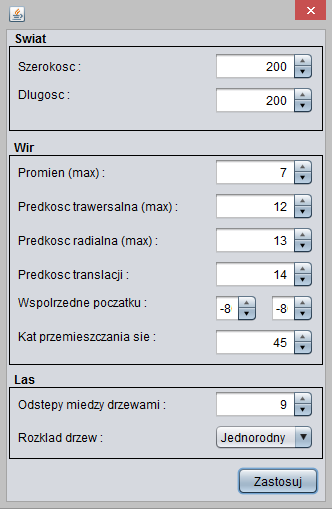
\includegraphics[scale=0.7]{test1p}
	\caption{Parametry pierwszej przykładowej symulacji.}
	\label{fig:test1p}
\end{figure} 

Wyniki symulacji zaprezentowane są na rysunku~\ref{fig:test1}. Jak widzimy, zgodnie z założeniami modelu tornado dokonało największych zniszczeń na obrzeżach lasu, gdzie wytrzymałości drzew są najmniejsze. Najlepiej przetrwały drzewa centralne, które otoczone są innymi drzewami.

\begin{figure}[!h]
	\center
	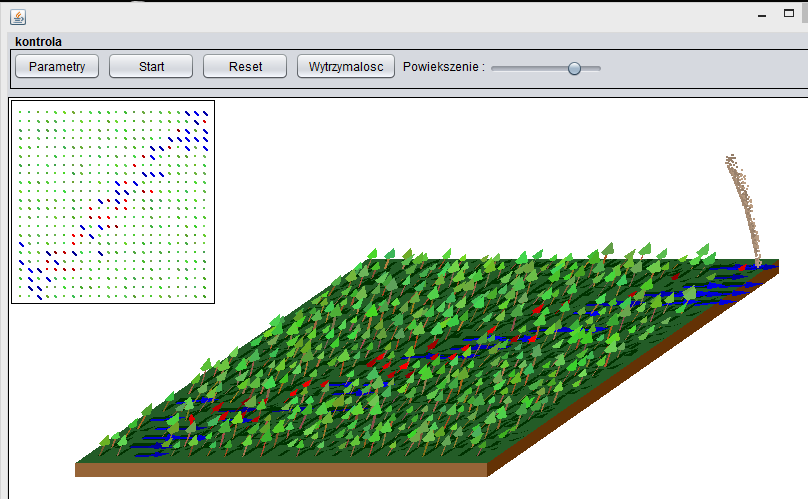
\includegraphics[scale=0.62]{test1}
	\caption{Wynik pierwszej przykładowej symulacji.}
	\label{fig:test1}
\end{figure} 

\subsection{Symulacja szarokiego tornada}

Parametry drugiej symulacji przedstawione są na rysunku~\ref{fig:test2p}. Jest to dosyć szersze tornado, o parametrach podobnych do pierwszego przykładu.

\begin{figure}[!h]
	\center
	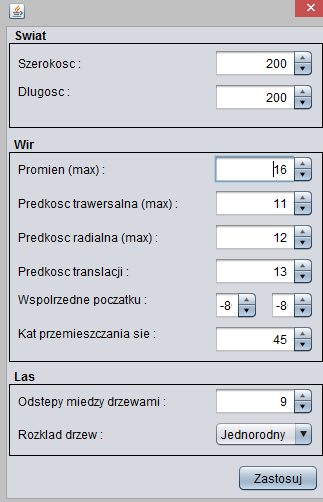
\includegraphics[scale=0.7]{test2p}
	\caption{Parametry drugiej przykładowej symulacji.}
	\label{fig:test2p}
\end{figure} 

Wyniki symulacji zaprezentowane są na rysunku~\ref{fig:test2}. Można zauważyć, iż tornado ma większy zasięg, jednak zwiększył się stosunek ilości drzew złamanych do ilości drzew przewróconych, co wskazuje na mniejszą siłę wiatru. Również w centrum tornada część drzew zostało nietkniętych, ponieważ w środku tornada panuje mniejszy wiatr. Tak jak w pierwszym przypadku można zaobserwować zmniejszoną wytrzymałość drzew na krańcach lasu.

\begin{figure}[!h]
	\center
	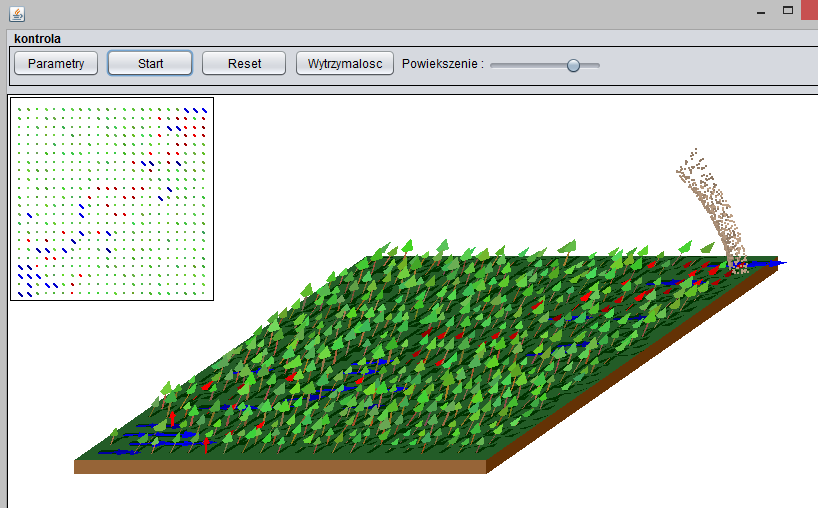
\includegraphics[scale=0.62]{test2}
	\caption{Wynik drugiej przykładowej symulacji.}
	\label{fig:test2}
\end{figure} 

\section{Walidacja}

Poddając model walidacji można się przekonać, czy wybrany model wiernie odwzorowuje rzeczywiste zjawiska fizyczne.
Zdjęcie~\ref{fig:walid1} przedstawia las po przejściu tornada w Hrabstwiw Rabun w stanie Georgia w Stanach Zjednoczonych. Można zauważyć, że tornado miało dużą szerokość, czym przypominało tornado z drugiej przykładowej symulacji. Widać także podobieństwo w skutkach -- oba tornada w przeważającej ilości tylko połamały drzewa, ponieważ nie posiadały wystarczającej siły aby je przewrócić.

\begin{figure}[!h]
	\center
	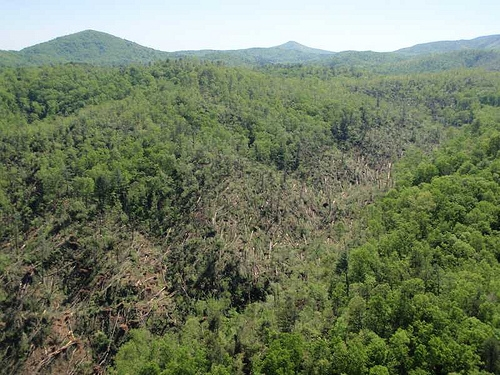
\includegraphics[scale=0.75]{walid1}
	\caption{Las po tornadzie w stanie Georgia.}
	\label{fig:walid1}
\end{figure} 

Zdjęcie~\ref{fig:walid2} ukazuje las w Parku Narodowmy Great Smoky Mountains na pograniczu stanów Karolina Północna i Tennessee w Stanach Zjednoczonych po przejściu tornada. Widać, że tornado miało większą siłę i było momentami stosunkowo wąskie. Tam, gdzie trzewa rosły rzadziej, tornado wyrządziło największe szkody. Na zewnątrz centrum tornada zostały wyrządzone większe szkody niż na trasie środka wiru. Można uznać, że dane te zgadzają się z przyjętym modelem.

\begin{figure}[!h]
	\center
	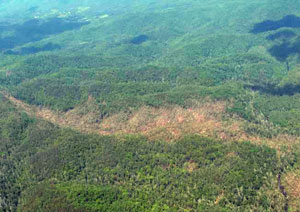
\includegraphics[scale=0.75]{walid2}
	\caption{Las po tornadzie w Parku Narodowmy Great Smoky Mountains.}
	\label{fig:walid2}
\end{figure} 